\documentclass{article}
\usepackage{listings}
\usepackage{listings}
\usepackage{xcolor}
\usepackage{algorithm}
\usepackage{algpseudocode}
\definecolor{codegreen}{rgb}{0,0.6,0}
\definecolor{codegray}{rgb}{0.5,0.5,0.5}
\definecolor{codepurple}{rgb}{0.58,0,0.82}
\definecolor{backcolour}{rgb}{0.95,0.95,0.92}

\lstdefinestyle{code}{
    backgroundcolor=\color{codegray},
    basicstyle=\ttfamily\footnotesize,
    keywordstyle=\color{codeblue},
    commentstyle=\color{red},
    stringstyle=\color{red},
    basicstyle=\ttfamily\footnotesize,
    breakatwhitespace=false,         
    breaklines=true,                 
    captionpos=b,                    
    keepspaces=true,                 
    numbers=left,                    
    numbersep=5pt,                  
    showspaces=false,                
    showstringspaces=false,
    showtabs=false,                  
    tabsize=2
}

\definecolor{codegray}{gray}{0.9}
\definecolor{codeblue}{rgb}{0.0, 0.0, 0.5}

\lstset{style=code}
% Language setting
% Replace `english' with e.g. `spanish' to change the document language
\usepackage[english]{babel}

% Set page size and margins
% Replace `letterpaper' with `a4paper' for UK/EU standard size
\usepackage[letterpaper,top=2cm,bottom=2cm,left=4cm,right=4cm,marginparwidth=1.75cm]{geometry}

% Useful packages
\usepackage{amsmath}
\usepackage{graphicx}
\usepackage[colorlinks=true, allcolors=blue]{hyperref}


\title{Operations Reserach 2 Final Thesis}
\author{Youssef Ben Khalifa}

\begin{document}
\maketitle

\tableofcontents

\cleardoublepage

\listofalgorithms
\addcontentsline{toc}{section}{List of Algorithms}

\cleardoublepage

\section{Introduction}
The Traveling Salesman Problem (TSP) stands as one of the most iconic and extensively studied problems in combinatorial optimization and computer science. Despite its deceptively simple formulation—finding the shortest 
possible route that visits each city exactly once and returns to the origin city—the TSP has profound implications for both theoretical computer science and practical applications.

In this thesis we will go over the implementation of the main heuristics involving the famous TSP problem. The entire implementation is done using the C programming language and the 
CPLEX optimization LP optimization framework.
The goal is to research and implement the most common Metaheuristics and Mathheuristics for solving the TSP problem using MIP problems.

Throughout this thesis, we will explore the historical development of each optimization method discussed. We will trace the evolution of metaheuristics from early construction heuristics to 
sophisticated approaches like 
Tabu Search and Variable Neighborhood Search, examining how these methods emerged in response to computational challenges. 
Similarly, we will investigate the historical context behind mathheuristics, which represent a 
more recent fusion of mathematical programming with heuristic frameworks, developed to address the 
limitations of pure exact methods when tackling large-scale combinatorial problems. This historical perspective will 
provide valuable insights into why particular techniques were developed and how they have evolved to their current form.


\subsection{The TSP Problem and Its Significance}
The TSP belongs to the class of NP-hard problems, meaning that no known algorithm can solve it optimally in polynomial time as the problem size increases. 
This fundamental hardness has made the TSP a benchmark problem for evaluating algorithmic approaches and computational methods. The significance of the TSP extends far beyond its theoretical interest, with applications 
spanning numerous domains:
\begin{itemize}
	\item Logistics and transportation planning
	\item Circuit board drilling in manufacturing
	\item DNA sequencing in bioinformatics
	\item Vehicle routing and delivery optimization
	\item Telecommunications network design
	\item Warehouse order picking
\end{itemize}

The ubiquity of the TSP in real-world applications has spurred extensive research into its solution methods, 
leading to a rich body of literature that encompasses exact algorithms, heuristics, and metaheuristics.

\subsection{Heuristics and Metaheuristics for TSP}
Given the computational intractability of finding exact solutions for large TSP instances, researchers have developed various metaheuristics—high-level problem-independent algorithmic frameworks 
that provide strategies for developing heuristic optimization algorithms. Unlike exact methods, metaheuristics sacrifice the guarantee of optimality for computational efficiency, providing near-optimal solutions in reasonable time frames.

Metaheuristics for the TSP include:
\begin{itemize}
	\item Construction heuristics like Nearest Neighbor and Greedy algorithms that build tours incrementally
	\item Local search methods such as 2-opt and 3-opt that iteratively improve solutions
	\item Population-based approaches like Genetic Algorithms that evolve multiple solutions simultaneously
	\item Memory-based techniques such as Tabu Search that use historical information to guide the search
	\item Adaptive methods like GRASP (Greedy Randomized Adaptive Search Procedure) that combine greedy elements with randomization
\end{itemize}

These approaches have proven remarkably effective in practice, often producing solutions within a few percentage points of optimality for instances with thousands of cities.

\subsection{Mathheuristics for TSP}
Mathheuristics represent a more recent development in the field, combining mathematical programming techniques with metaheuristic frameworks. 
These hybrid methods leverage the strengths of exact optimization methods (like linear and integer programming) while maintaining the scalability advantages of heuristics.

For the TSP, mathheuristics typically involve:
\begin{itemize}
	\item Decomposition techniques that break the problem into manageable subproblems
	\item Variable fixing approaches that reduce the problem size by fixing certain decision variables
	\item Local branching methods that explore neighborhoods defined by mathematical constraints
	\item Cut generation procedures that iteratively strengthen mathematical formulations
\end{itemize}

By integrating mathematical rigor with heuristic flexibility, mathheuristics often achieve superior performance compared to either approach used independently, 
especially for complex or large-scale instances.

\subsection{Scope of This Thesis}
This thesis investigates both traditional metaheuristics and modern mathheuristics for solving the TSP, implementing and analyzing several 
approaches using the C programming language and the CPLEX optimization framework. We focus on understanding the mathematical foundations, implementation details, 
and computational performance of these methods, with particular attention to their practical effectiveness across different problem instances.

Through systematic experimentation and analysis, we aim to provide insights into the strengths and limitations of different solution approaches, contributing to the 
ongoing effort to develop more efficient algorithms for this foundational optimization problem.

Throught the next chapters we will be going over following:
\begin{enumerate}
	\item \textbf{Introduction to the TSP Problem}: quick overview of the Mathematical formulation of the TSP problem.
	\item \textbf{Heuristics}: Implementation of common heuristic algorithms including:
		\begin{itemize}
			\item Greedy Randomized Adaptive Search (GRASP)
			\item Extra Mileage
			\item Refining Heuristics (2-opt move)
		\end{itemize}
	\item \textbf{Neighbourhood Search}: Implementation of neighbourhood search algorithms including:
		\begin{itemize}
			\item Tabu Search
			\item Variable Neighborhood Search (VNS)
		\end{itemize}
	\item \textbf{Mathheuristics}: Implementation of mathematical optimization techniques combined with heuristics:
		\begin{itemize}
			\item Hard Fixing
			\item Local Branching
		\end{itemize}
\end{enumerate}

For each algorithm, we will examine the implementation details, mathematical foundations, and effectiveness in solving the TSP problem. 
The implementations for the mathheuristic algorithms are done utilizing the CPLEX optimization framework. 

\newpage

\section{The Traveling Salesman Problem}
The Traveling Salesman Problem (TSP) is one of the most extensively studied problems in combinatorial optimization. The problem asks to find the shortest possible route that visits each city exactly once and returns to the origin city, 
given a set of cities and the distances between them.
Formally, given a set of $n$ cities and a cost matrix $[cij]$ that specifies the cost (or distance) of traveling from city $i$ to city $j$, the goal is to find a permutation of the cities that minimizes the total tour length. 
Despite its simple description, the TSP is NP-hard, meaning there is no known polynomial-time algorithm that can solve it optimally for large instances.

\subsection{History of the TSP}
The Travelling salesman problem was first formulated in the 1930's, whose first mathematical formul was given my Meril M. Flood.
Since its introduction, the TSP problem has been one of the most researched subject in the mathematical optimization filed, and since then it has served
as a benchmark for many optimization algorithms.
Throughout the years, several exact approaches have been developed that are able to compute an exact solution even for very large instances of 
the problem (Applegate, Bixby, Chvatal, Cook, \& Problem, 2006), and also many heuristic approaches have been proposed that approximate with incredible 
accuracy even instances with milions of nodes.  

Numerous research efforts—such as those by Chisman (1975), Garg \& Ravi (2000), and Henry-Labordere (1969)—highlight the strong academic 
interest in extensions and variants of the Traveling Salesman Problem (TSP). Over the years, several important extensions have been explored, 
including:
\begin{itemize}
	\item the Vehicle Routing Problem (Laporte, 1992),

	\item he TSP with Time Windows (da Silva \& Urrutia, 2010),
	
	\item the Steiner TSP (Rodríguez-Pereira, Fernández, Laporte, Benavent, \& Sykora, 2019),
	
	\item the Selective TSP (Laporte \& Martello, 1990),
	
	\item the Multi-objective TSP (Psychas, Delimpasi, \& Marinakis, 2015),
	
	\item the Multiple TSP (Cheikhrouhou \& Khoufi, 2021),
	
	\item the Bottleneck TSP (Garfinkel \& Gilbert, 1978),
	
	\item the Prize Collecting TSP (Balas, 1989),
	
	\item the Clustered TSP (Chisman, 1975), and
	
	\item the Generalized TSP (Henry-Labordere, 1969; Saskena, 1970; Srivastava, Kumar, Garg, \& Sen, 1969).
\end{itemize}


These extensions reflect the versatility and practical significance of the TSP framework across a wide range of optimization scenarios.

\subsection{Mathematical Formulation}
First let us define the components that characterize the TSP problem: we begin from a graph $G = (V, E)$ where $V$ is the set of vertices (cities) and $E$ is the set of edges connecting the vertices, and a cost matrix $C$ containing the weights/costs of each edge $(i, j) \in E$. 
Spoiler: in the implementation instead of adopting a big cost matrix, we will be simply using the euclidean distance between the nodes for computing the cost $c_{i, j}$ of a given edge $(i, j)$ , therefore the cost of a tour will simply be computed as the sum of the euclidean distances between the nodes. This will not affect the final formulation.   

We then can formalize the Traveling Salesman Problem as an optimization problem. The objective is to find a Hamiltonian cycle (a closed path visiting each vertex exactly once) of minimum total cost. Below we present two common mathematical formulations:

\subsubsection{Miller-Tucker-Zemlin (MTZ) Formulation}
This formulation uses additional variables to prevent subtours:
\begin{equation}
	\min \sum_{i=1}^{n} \sum_{j=1}^{n} c_{ij} x_{ij}
\end{equation}
subject to:
\begin{equation}
	\sum_{j=1}^{n} x_{ij} = 1 \quad \forall i \in \{1, \ldots, n\}
\end{equation}
\begin{equation}
	\sum_{i=1}^{n} x_{ij} = 1 \quad \forall j \in \{1, \ldots, n\}
\end{equation}
\begin{equation}
	u_i - u_j + nx_{ij} \leq n-1 \quad \forall i,j \in \{2, \ldots, n\}, i \neq j
\end{equation}
\begin{equation}
	1 \leq u_i \leq n-1 \quad \forall i \in \{2, \ldots, n\}
\end{equation}
\begin{equation}
	x_{ij} \in \{0, 1\} \quad \forall i, j \in \{1, \ldots, n\}
\end{equation}
where:
\begin{itemize}
	\item $c_{ij}$ is the cost of traveling from node $i$ to node $j$.
	\item $x_{ij}$ is a binary variable that indicates whether the salesman travels from node $i$ to node $j$.
	\item $u_i$ is a continuous variable that represents the position of node $i$ in the tour (node 1 is considered the starting point).
\end{itemize}

\subsubsection{Dantzig-Fulkerson-Johnson (DFJ) Formulation}
This alternative formulation uses subtour elimination constraints:
\begin{equation}
	\min \sum_{i=1}^{n} \sum_{j=1}^{n} c_{ij} x_{ij}
\end{equation}
subject to:
\begin{equation}
	\sum_{j=1}^{n} x_{ij} = 1 \quad \forall i \in \{1, \ldots, n\}
\end{equation}
\begin{equation}
	\sum_{i=1}^{n} x_{ij} = 1 \quad \forall j \in \{1, \ldots, n\}
\end{equation}
\begin{equation}
	\sum_{i \in S} \sum_{j \in S} x_{ij} \leq |S| - 1 \quad \forall S \subset \{1, \ldots, n\}, 2 \leq |S| \leq n-1
\end{equation}
\begin{equation}
	x_{ij} \in \{0, 1\} \quad \forall i, j \in \{1, \ldots, n\}
\end{equation}

In this formulation, the third constraint eliminates subtours by ensuring that for any subset $S$ of vertices, the number of edges in the solution connecting vertices within $S$ must be at most $|S|-1$. This prevents the formation of isolated cycles within the subset.

The main challenge with the DFJ formulation is that it contains an exponential number of constraints ($2^n - 2 - n$ subtour elimination constraints). In practice, these constraints are typically added dynamically through a branch-and-cut approach, which we will explore later in the CPLEX implementation section.

For symmetric TSP problems (where $c_{ij} = c_{ji}$), we can simplify the formulation by defining variables only for $i < j$ and adjusting the constraints accordingly.


\newpage

\section{Development and environment setup}
All the code implementations mentioned in this thesis have been developed and tested on a Linux environment using the C programming language. The main components of the development setup are:

\paragraph{System Environment}
\begin{itemize}
	\item Operating System: Ubuntu 22.04 LTS
	\item Architecture: x86\_64
	\item Compiler: GCC 11.4.0
	\item Build System: CMake 3.22.1
\end{itemize}

\paragraph{Dependencies}
\begin{itemize}
	\item IBM ILOG CPLEX Optimization Studio 22.1.1
	\item Standard C Libraries (stdio.h, stdlib.h, math.h)
	\item Python 3.8 or higher (for profiling and testing)
\end{itemize}

\paragraph{Project Structure}
The project is organized as follows:
\begin{itemize}
	\item \texttt{/src}: Contains all source files
	\item \texttt{/include}: Header files
	\item \texttt{/test}: Test instances and test cases
	\item \texttt{/build}: Build directory (generated by CMake)
	\item \texttt{/profiler}: Profiling scripts and results
\end{itemize}

\paragraph{Build Configuration}
The project uses CMake as its build system. The main CMakeLists.txt file configures the build environment and links necessary dependencies, 
particularly the CPLEX libraries required for the mathematical optimization components.

\subsection{Data Structures}
The implementation uses several key data structures to efficiently manage and process TSP-related data:

\subsubsection{TSP Instance Structure}
The core data structure is the \texttt{instance} struct, which holds all problem-related data:
\begin{lstlisting}[language=C, caption={TSP Instance Structure}]
typedef struct {
	int nnodes;          // number of nodes
	double* xcoord;      // x coordinates of nodes
	double* ycoord;      // y coordinates of nodes
	int* solution;       // current solution tour
	double best_cost;    // cost of best solution found
	double elapsed_time; // computational time
} instance;
\end{lstlisting}

\subsubsection{Solution Representation}
the TSP solutions are represented in two main ways:
\begin{enumerate}
	\item Solution structure for exact methods:
	\begin{itemize}
		\item Contains an integer array (solution->solution) that stores the sequence of nodes to visit in order
		\item Each element in the array represents a city index (0-based)
		\item Used by methods like GRASP, Extra Mileage, and Tabu Search
	\end{itemize}
	\item CPLEX representation for exact methods:
	\begin{itemize}
		\item Uses a binary variable array (xstar) where each element represents whether an edge is used
		\item Edge variables are indexed using \texttt{get\_cplex\_variable\_index(i, j, inst)}
		\item When a CPLEX solution is found, it's converted to the sequence representation using \texttt{build\_solution()}
	\end{itemize}
\end{enumerate}

The \texttt{build\_solution()} function takes the binary edge variables from CPLEX and constructs a tour sequence by finding connected components. 
The final result is always a permutation of nodes (0 to n-1) representing the order to visit cities in the TSP tour.


\cleardoublepage

\section{Heuristics for TSP}
Metaheuristics represent a sophisticated class of computational methods that have evolved to address complex optimization problems where exact methods become impractical due to computational constraints. 
As optimization problems grow in scale and complexity, traditional exact methods often struggle with the combinatorial explosion of possible solutions. 
Metaheuristics emerged as an effective approach to navigate these vast solution spaces by intelligently balancing exploration of new regions with exploitation of promising areas.
In this section we will go over a brief history of the development of the metaheuristics algorithms and the implementation of the following metaheuristics:
\begin{itemize}
	\item Greedy Randomized Adaptive Search (GRASP)
	\item Extra Mileage
	\item Refining Heuristics (2-opt move)
\end{itemize}
for each algorihtm you will see the pseudocode for both the algorithm and the implementation of the algorithm in C.


\subsection{Greedy Randomized Adaptive Search (GRASP)}
The GRASP method is basically a greedy randomized adaptive search procedure.
It consists of two main phases: construction and local search.
In the construction phase, a feasible solution is built, one element at a time, in a greedy randomized fashion.
In the local search phase, the neighborhood of the constructed solution is explored until a local minimum is found.

\paragraph{Construction Phase}
In the construction phase, the solution is built iteratively. At each iteration, a candidate list is created,
containing the best elements to be added to the solution. One of these elements is chosen randomly, according
to a probability distribution, and added to the solution.

\paragraph{Local Search Phase}
In the local search phase, the algorithm explores the neighborhood of the constructed solution to find a local minimum.
This is done by iteratively replacing the current solution with a better solution from its neighborhood,
until no better solution can be found.

\paragraph{Algorithm}
The GRASP algorithm can be summarized as follows:
\begin{enumerate}
	\item \textbf{Initialization:} Set the best solution found to null.
	\item \textbf{Construction:} Build a feasible solution using the greedy randomized approach.
	\item \textbf{Local Search:} Improve the constructed solution using local search.
	\item \textbf{Update:} If the improved solution is better than the best solution found, update the best solution.
	\item \textbf{Termination:} Repeat steps 2-4 until a stopping criterion is met (e.g., a maximum number of iterations).
\end{enumerate}

\newpage
\begin{algorithm}[!ht]
\caption{TSP GRASP Metaheuristic}
\begin{algorithmic}[1]
\Procedure{TSP\_GRASP}{instance, max\_iterations}
\State best\_solution $\gets$ null
\State best\_cost $\gets \infty$

\For{iteration $\gets$ 1 \textbf{to} max\_iterations}
	\State // Construction Phase
	\State solution $\gets \emptyset$
	\State current $\gets$ RandomStartNode()
	\State solution.Add(current)
	
	\While{|solution| < n}
		\State candidates $\gets$ BuildCandidateList(current)
		\State RCL $\gets$ BuildRestrictedCandidateList(candidates)
		\State next $\gets$ RandomSelect(RCL)
		\State solution.Add(next)
		\State current $\gets$ next
	\EndWhile
	
	\State // Local Search Phase
	\State improved\_solution $\gets$ LocalSearch(solution)
	\State cost $\gets$ ComputeCost(improved\_solution)
	
	\If{cost < best\_cost}
		\State best\_solution $\gets$ improved\_solution
		\State best\_cost $\gets$ cost
	\EndIf
\EndFor

\State \Return best\_solution
\EndProcedure
\end{algorithmic}
\end{algorithm}


\paragraph{Implementation}
The implementation of the GRASP algorithm takes as input arguments:
\begin{itemize}
	\item \texttt{instance}: The TSP instance data structure.
	\item \texttt{start\_node}: The index of the starting node for the tour.
\end{itemize}
The function internally allocates and sets the solution as an array integers representing the tour....
The GRASP algorithm is implemented as follows:
\begin{enumerate} 
	\item \textbf{Setup}:
	      \begin{itemize}
		      \item The function initializes the current node index to the starting node (which is passed as an argument) 
			  and sets the remaining nodes count to the total number of nodes.
		      \item It allocates memory for the solution array and remaining nodes arrays. These two arrays will be used respectively to store the tour and the remaining nodes for the main loop to visit.
		      \item The solution array is initialized with \texttt{-1} to indicate that no nodes have been visited yet.
		      \item The remaining nodes array is initialized with all node indices.
	      \end{itemize}

	\item \textbf{Main Loop}:
	      \begin{itemize}
		      \item The function iterates over all nodes to construct the solution.
		      \item For each node, it finds the nearest unvisited node using the \texttt{euclidean\_nearest\_node} function.
		      \item If no nearest node is found (i.e., all nodes are visited), it connects the current node back to the starting node to complete the tour.
		      \item Otherwise, it updates the solution with the nearest node and logs the current node index and nearest node found.
		      \item The current node index is updated to the nearest node for the next iteration.
	      \end{itemize}
		

	\item \textbf{Finalization}:
	      \begin{itemize}
		      \item After constructing the solution, the function records the end time and calculates the elapsed time.
		      \item It logs the total time taken and the cost of the solution.
		      \item Finally, it frees the allocated memory for the remaining nodes array.
	      \end{itemize}
\end{enumerate}

Here's the pseudocode of the implementation:

\begin{algorithm}[!ht]
\caption{TSP GRASP}
\begin{algorithmic}[1]
\Procedure{TSP\_GRASP}{instance, solution, alpha}
\State solution $\gets \emptyset$
\State candidates $\gets$ \{1, ..., n\} \Comment{Set of unvisited nodes}
\State current $\gets$ RandomNode(candidates)
\State solution.Add(current)
\State Remove(candidates, current)

\While{candidates not empty}
    \State RCL $\gets \emptyset$ \Comment{Restricted Candidate List}
    \State $c_{min} \gets$ MinDistance(current, candidates)
    \State $c_{max} \gets$ MaxDistance(current, candidates)
    \State threshold $\gets c_{min} + \alpha(c_{max} - c_{min})$
    
    \ForAll{node $\in$ candidates}
        \If{Distance(current, node) $\leq$ threshold}
            \State RCL.Add(node)
        \EndIf
    \EndFor
    
    \State next $\gets$ RandomSelect(RCL)
    \State solution.Add(next)
    \State Remove(candidates, next)
    \State current $\gets$ next
\EndWhile

\State solution.Add(solution[0]) \Comment{Return to starting node}
\State \Return solution
\EndProcedure
\end{algorithmic}
\end{algorithm}

\newpage

\subsection{Extra Mileage}
In the extra mileage heuristic, we try to build a valid tsp solution starting an edge of the graph and we try and build a 
tour by selecting the adjacent edge with the minimum cost.

\paragraph{Algorithm}
The extra mileage algorithm can be summarized as follows:
\begin{enumerate}
	\item \textbf{Initialization:} Initialize the starting edge.
	\item \textbf{Construction:} Build a feasible solution by iteratively selecting the edge with the minimum cost.
	\item \textbf{Update:} If the improved solution is better than the best solution found, update the best solution.
	\item \textbf{Termination:} Repeat steps 2-3 until a stopping criterion is met (e.g., a maximum number of iterations).
\end{enumerate}

\paragraph{Implementation}
The extra mileage algoithm implementation takes as input arguments:
\begin{itemize}
	\item \texttt{instance}: The TSP instance data structure.
	\item \texttt{starting\_pair}: The pair of nodes that will be used to start the tour.
\end{itemize}
Ideally the starting pair should be the most distant pair of nodes in the graph in order to optimize the construction of the solution,
by design this is not a restriction that has been instrisically implemented into the function, so any pair of nodes can be used as a starting pair.
The extra mileage algorithm is implemented as follows:
\begin{enumerate} 
	\item \textbf{Setup}:
	\begin{itemize}
		\item The function initializes the current\_pair to the starting pair (which is passed as an argument).
		\item An heuristic state data stcuture is initialized to keep the track of the covered nodes and the final solution 
	\end{itemize}
	\item \textbf{Main Loop}:
	      \begin{itemize}
		      \item While there are uncovered nodes (condition based on the comparison of the covered nodes count and the total number of nodes), 
			  the function iterates over the uncovered nodes to construct the solution:
		            \begin{itemize}
			            \item For each covered node, a second loop is exectued to find the nearest uncovered node such that 
			            the the resulting edge between the two nodes is the argument that minimizes the total cost of the tour up until that point.
			            \item if such node is found, that node is selected and added to the tour, 
						the covered nodes count is incremented and the node is removed from the uncovered nodes list.
		            \end{itemize}
	      \end{itemize}
		
	\item \textbf{Finalization}:
	      \begin{itemize}
		      \item Once all nodes are covered, the function calculates the total cost of the solution.
		      \item It records the end time and calculates the elapsed time.
	      \end{itemize}
\end{enumerate}

\newpage

\begin{algorithm}[!ht]
\caption{TSP Extra Mileage}
\begin{algorithmic}[1]
\Procedure{TSP\_ExtraMileage}{instance, solution, start\_pair}
\State solution $\gets \emptyset$
\State candidates $\gets$ \{1, ..., n\} \Comment{Set of unvisited nodes}
\State tour $\gets$ [start\_pair.first, start\_pair.second] \Comment{Initial tour with farthest pair}
\State Remove(candidates, start\_pair.first)
\State Remove(candidates, start\_pair.second)

\While{candidates not empty}
    \State best\_node $\gets$ null
    \State best\_pos $\gets$ null
    \State min\_cost $\gets \infty$

    \ForAll{node $\in$ candidates}
        \ForAll{pos $\in$ \{1, ..., |tour|\}}
            \State extra\_dist $\gets$ Distance(tour[pos-1], node)
            \State extra\_dist $\gets$ extra\_dist + Distance(node, tour[pos])
            \State extra\_dist $\gets$ extra\_dist - Distance(tour[pos-1], tour[pos])
            
            \If{extra\_dist < min\_cost}
                \State min\_cost $\gets$ extra\_dist
                \State best\_node $\gets$ node
                \State best\_pos $\gets$ pos
            \EndIf
        \EndFor
    \EndFor

    \State Insert(tour, best\_node, best\_pos)
    \State Remove(candidates, best\_node)
\EndWhile

\State solution $\gets$ tour
\State \Return solution
\EndProcedure
\end{algorithmic}
\end{algorithm}

\newpage

\section{Refining Heuristics}
Refining heuristics are a type of heuristic algorithm that iteratively improve an initial solution by applying a series of local search moves. These can be applied on top of the existing heuristics we have 
introduced so far in order to improve their performance. In the next section we will go over a one particular refining heuristic called the \textit{2-opt move}\cite{Heuristics_for_the_Traveling_Salesman_Problem}.

\subsection{2-opt Move}
Assume we have a graph $G = (V, E)$ and a directed tour $T \subseteq E$, valid as a tsp solution, 
the 2-opt move takes two edges in that tour and swaps the nodes 
between them.  In particular, let $(i, j), (h, k) \in T$, the 2-opt move replaces the edges $(i, j)$ and $(h, k)$ with the edges $(i, h)$ and $(j, k)$. \\
\\
\paragraph{Algorithm}
The goal of this type of operation is to swap two "longer" edges for two "shorter" ones (by "longer" and "shorter" we refer to the edge cost): 
therefore in our refining heuristic we aim at:
\begin{enumerate}
	\item Selecting two edges $(i, j), (h, k) \in T$: for selecting the two edges we can adopt two different strategies:
	\begin{itemize}
		\item Select the first pair of edges that satisfy the following:
		\begin{equation}
			c_{G}(i, j) + c_{G}(h, k) > c_{G}(i, h) + c_{G}(j, k)
			\label{eq:2-opt-move}
		\end{equation}
		\item Or select the pair of edges in $G$ which swap results in the maximum cost reduction:
		\begin{equation}
			\arg\max_{((i, j), (h, k)) \in E \times E} \Delta c_G ((i, j), (h, k))
			\label{eq:2-opt-move-argmax}
		\end{equation}
		with 
		\begin{equation}
			\Delta c_G((i, j), (h, k)) = (c_G(i, h) + c_G(j, k)) - (c_G(i, j) + c_G(h, k))
		\end{equation}
	\end{itemize}
	
	where $c_G(i, j)$ is the cost associated with edge $(i, j)$.
	\item Replacing the two edges with the edges $(i, h)$ and $(j, k)$.
	\item If the graph is directed, invert the direction of the tour of the edges between $(j, k)$ and $(i, h)$.
\end{enumerate}
\paragraph{Implementation}
The 2-opt move implementation takes as input arguments:
\begin{itemize}
	\item \texttt{instance}: an instance of the TSP problem so solve.
	\item \texttt{solution}: an instance of a valid TSP solution.
\end{itemize}
The function is implemented as follows:
\begin{enumerate}
	\item \textbf{Main loop:} 
	\begin{itemize}
	\item The function iterates over all edges in the solution to find a valid 2-opt move. In this implementations, this is identified by the pair of edges that satisfy (\ref{eq:2-opt-move-argmax})
	\item If a valid 2-opt move is found, the pair is saved as the designated edges to be swapped.
	\end{itemize}
	\item \textbf{Swap:} We apply the 2-opt move on the solution by swapping the designated edges.
	\item \textbf{Finalization:} We invert the direction of the edges between $(j, k)$ and $(i, h)$ if the graph is directed.
\end{enumerate}
\newpage
\begin{algorithm}[!ht]
\caption{TSP 2-opt Local Search}
\begin{algorithmic}[1]
\Procedure{TSP\_TwoOpt}{instance, solution}
\State improved $\gets$ true
\While{improved}
    \State improved $\gets$ false
    \State best\_gain $\gets$ 0
    \State best\_i $\gets$ -1
    \State best\_j $\gets$ -1

    \For{i $\gets$ 0 \textbf{to} n-2}
        \For{j $\gets$ i+1 \textbf{to} n-1}
            \State gain $\gets$ CalculateTwoOptGain(i, j)
            \If{gain < best\_gain}
                \State best\_gain $\gets$ gain
                \State best\_i $\gets$ i
                \State best\_j $\gets$ j
                \State improved $\gets$ true
            \EndIf
        \EndFor
    \EndFor

    \If{improved}
        \State ReversePath(solution, best\_i+1, best\_j)
    \EndIf
\EndWhile

\State \Return solution
\EndProcedure

\Function{CalculateTwoOptGain}{i, j}
    \State old\_dist $\gets$ Distance(tour[i], tour[i+1])
    \State old\_dist $\gets$ old\_dist + Distance(tour[j], tour[j+1])
    \State new\_dist $\gets$ Distance(tour[i], tour[j])
    \State new\_dist $\gets$ new\_dist + Distance(tour[i+1], tour[j+1])
    \State \Return new\_dist - old\_dist
\EndFunction
\end{algorithmic}
\end{algorithm}

\newpage

\section{Metaheuristics for the TSP}
Metaheuristics represent a sophisticated evolution from classical heuristic approaches in solving the Traveling Salesman Problem (TSP). 
While traditional heuristics typically follow a fixed set of rules to construct or improve solutions, metaheuristics employ more dynamic 
and adaptive strategies to explore the solution space effectively.

The key distinctions between classical heuristics and metaheuristics are:

\begin{itemize}
	\item \textbf{Search Strategy}: Classical heuristics often follow a deterministic path, while metaheuristics incorporate randomization and adaptive mechanisms to escape local optima.
	
	\item \textbf{Solution Quality}: Traditional heuristics may get stuck in local optima, whereas metaheuristics employ various techniques (like perturbation or memory structures) to find better solutions.
	
	\item \textbf{Computational Complexity}: Classical heuristics typically have lower computational requirements but may produce inferior solutions compared to metaheuristics.
	
	\item \textbf{Flexibility}: Metaheuristics can be adapted to various problem types and instances, while classical heuristics are often problem-specific.
\end{itemize}

Common metaheuristic approaches for the TSP include:
\begin{itemize}
	\item \textbf{Tabu Search}: Uses memory structures to avoid revisiting recent solutions
	\item \textbf{Variable Neighborhood Search}: Systematically changes neighborhood structures to escape local optima
	\item \textbf{Simulated Annealing}: Employs probabilistic acceptance of worse solutions
	\item \textbf{Genetic Algorithms}: Evolves solutions through selection and recombination operations
\end{itemize}

These methods have proven particularly effective for large-scale TSP instances where exact methods become computationally infeasible.

\subsection{Tabu Search}
The Tabu search is a type of neighborhood search algorithm. 
Differently with what happened with greedy algorithms like the GRASP, the Tabu search algorithm is able to escape local optima by allowing the search to move to worse solutions,
which can help the algorithm explore new regions of the search space and potentially find better solutions.
The main idea behind the Tabu search heuristic is to exclude the already explored solutions from the search space. 
This is done by maintaining a tabu list that stores the solutions that have been visited recently. 
The tabu list is used to prevent the search from revisiting the same solutions, 
which can help the algorithm escape local optima and explore new regions of the search space\cite{Heuristics_for_the_Traveling_Salesman_Problem}.

\paragraph{Algorithm}
The Tabu search algorithm can be summarized as follows:
\begin{enumerate}
    \item \textbf{Initialization:} Initialize the tabu list and the best solution found.
    \item \textbf{Setup:} Initialize the current solution and the current iteration count.
    \item \textbf{Main Loop:} Repeat the following steps until a stopping criterion is met:
          \begin{itemize}
              \item Generate a set of candidate solutions by applying a set of moves to the current solution.
              \item Select the best candidate solution that is not in the tabu list.
              \item Update the tabu list with the selected solution.
              \item Update the current solution with the selected solution.
              \item If the selected solution is better than the best solution found, update the best solution.
              \item Increment the iteration count.
          \end{itemize}
    \item \textbf{Finalization:} Return the best solution found.
\end{enumerate}


\begin{algorithm}[!ht]
\caption{TSP Tabu Search}
\begin{algorithmic}[1]
\Procedure{TSP\_TabuSearch}{instance, initial\_solution, tabu\_size}
\State best\_solution $\gets$ initial\_solution
\State best\_cost $\gets$ ComputeCost(best\_solution)
\State current\_solution $\gets$ initial\_solution
\State tabu\_list $\gets$ EmptyQueue(tabu\_size)
\State iterations $\gets$ 0

\While{iterations < MAX\_ITERATIONS}
    \State best\_move $\gets$ null
    \State best\_gain $\gets \infty$
    
    \ForAll{i, j $\in$ PossibleMoves(current\_solution)}
        \If{(i, j) $\notin$ tabu\_list \textbf{or} AspirationCriteria()}
            \State gain $\gets$ CalculateSwapGain(i, j)
            \If{gain < best\_gain}
                \State best\_gain $\gets$ gain
                \State best\_move $\gets$ (i, j)
            \EndIf
        \EndIf
    \EndFor
    
    \State ApplyMove(current\_solution, best\_move)
    \State current\_cost $\gets$ ComputeCost(current\_solution)
    \State AddToTabuList(tabu\_list, best\_move)
    
    \If{current\_cost < best\_cost}
        \State best\_solution $\gets$ current\_solution
        \State best\_cost $\gets$ current\_cost
    \EndIf
    
    \State iterations $\gets$ iterations + 1
\EndWhile

\State \Return best\_solution
\EndProcedure
\end{algorithmic}
\end{algorithm}

\newpage

\subsection{Variable Neighbourhood Search}
The Variable Neighbourhood Search (VNS) heuristic is a metaheuristic that combines local search with a systematic change of neighbourhood structures. 
The idea is to explore different neighbourhoods of the current solution to escape local optima and find better solutions.
Many formulations and version for the VNS algorithm have been proposed in the literature, such as the \textit{Basic VNS}, \textit{Reduced VNS} and \textit{General VNS}.\cite{VariableNeighborhood_Search}\\

All of these forumlations are based on a neighbourhood search, which is defined within a solution space that can be explored using the \textit{two-opt move}, 
\textit{three-opt move} or the \textit{k-opt move}, depending on the general scheme of the algorithm. These operations that can be made in the solution space for the TSP problem allow to generate a neighborhood
starting from a given solution, each of which neighbour differ from one single \textit{2-opt move}\cite{Heuristics_for_the_Traveling_Salesman_Problem}. 

\paragraph{Algorithm}
In our imeplementation we will go over the General VNS scheme, in which the neighbours are simply generated from a single \textit{two-opt move}, and the \textit{shaking function} 
The VNS algorithm can be summarized as follows:
\begin{enumerate}
	\item \textbf{Initialization:} Initialize the current solution and the best solution found.
	\item \textbf{Setup:} Initialize the neighbourhood structure and the current iteration count.
	\item \textbf{Main Loop:} Repeat the following steps until a stopping criterion is met:
		  \begin{itemize}
			  \item Apply a local search algorithm to the current solution.
			  \item Generate a new solution by applying a perturbation to the current solution.
			  \item If the new solution is better than the current solution, update the current solution.
			  \item If the current solution is better than the best solution found, update the best solution.
			  \item Change the neighbourhood structure.
			  \item Increment the iteration count.
		  \end{itemize}
	\item \textbf{Finalization:} Return the best solution found.
\end{enumerate}
\begin{algorithm}
\caption{TSP Variable Neighborhood Search}
\begin{algorithmic}[1]
\Procedure{TSP\_VNS}{instance, initial\_solution, k\_max}
\State best\_solution $\gets$ initial\_solution
\State best\_cost $\gets$ ComputeCost(best\_solution)
\State k $\gets$ 1

\While{k $\leq$ k\_max}
    \State current\_solution $\gets$ best\_solution
    \State // Shaking phase
    \State current\_solution $\gets$ Shake(current\_solution, k)
    
    \State // Local search phase
    \State improved $\gets$ true
    \While{improved}
        \State improved $\gets$ false
        \State neighbor $\gets$ LocalSearch(current\_solution, k)
        \State neighbor\_cost $\gets$ ComputeCost(neighbor)
        
        \If{neighbor\_cost < ComputeCost(current\_solution)}
            \State current\_solution $\gets$ neighbor
            \State improved $\gets$ true
        \EndIf
    \EndWhile

    \If{ComputeCost(current\_solution) < best\_cost}
        \State best\_solution $\gets$ current\_solution
        \State best\_cost $\gets$ ComputeCost(current\_solution)
        \State k $\gets$ 1
    \Else
        \State k $\gets$ k + 1
    \EndIf
\EndWhile

\State \Return best\_solution
\EndProcedure

\Function{Shake}{solution, k}
    \For{i $\gets$ 1 \textbf{to} k}
        \State pos1, pos2 $\gets$ RandomPositions(solution.length)
        \State SwapNodes(solution, pos1, pos2)
    \EndFor
    \State \Return solution
\EndFunction
\end{algorithmic}
\end{algorithm}
\newpage

\subsection{Simulated Annealing}
Simulated Annealing (SA) is a probabilistic optimization algorithm inspired by the annealing process in metallurgy.
The algorithm is designed to find an approximate solution to optimization problems by exploring the solution space in a way that allows for both exploration and exploitation.
The key idea behind SA is to allow the algorithm to accept worse solutions with a certain probability,
which helps it escape local optima and explore the solution space more effectively.
\paragraph{Algorithm}
The Simulated Annealing algorithm can be summarized as follows:
\begin{enumerate}
	\item \textbf{Initialization:} Initialize the current solution, temperature, and cooling schedule.
	\item \textbf{Main Loop:} Repeat the following steps until a stopping criterion is met:
	      \begin{itemize}
		      \item Generate a new solution by applying a perturbation to the current solution.
		      \item Calculate the cost of the new solution.
		      \item If the new solution is better than the current solution, accept it.
		      \item If the new solution is worse than the current solution, accept it with a certain probability based on the temperature.
		      \item Update the temperature according to the cooling schedule.
	      \end{itemize}
	\item \textbf{Finalization:} Return the best solution found.
\end{enumerate}


\begin{algorithm}[!ht]
	\caption{Simulated Annealing for TSP}
	\begin{algorithmic}[1]
	\Procedure{SimulatedAnnealing}{instance, initial\_solution}
	\State $current\_solution \gets initial\_solution$
	\State $current\_cost \gets ComputeCost(current\_solution)$
	\State $best\_solution \gets current\_solution$
	\State $best\_cost \gets current\_cost$
	\State $temperature \gets initial\_temperature$
	\State $cooling\_rate \gets 0.95$
	\State $max\_iterations \gets 1000$
	
	\For{$i = 1$ to $max\_iterations$}
		\State Generate a random valid TSP solution $next\_solution$
		\State $new\_cost \gets ComputeCost(next\_solution)$
		
		\If{$new\_cost < current\_cost$}
			\State $current\_solution \gets next\_solution$
			\State $current\_cost \gets new\_cost$
			
			\If{$new\_cost < best\_cost$}
				\State $best\_solution \gets next\_solution$
				\State $best\_cost \gets new\_cost$
			\EndIf
		\Else
			\State $delta \gets new\_cost - current\_cost$
			\State $probability \gets e^{-delta / temperature}$
			\State $random \gets$ Random number between 0 and 1
			
			\If{$random < probability$}
				\State $current\_solution \gets next\_solution$
				\State $current\_cost \gets new\_cost$
			\EndIf
		\EndIf
		
		\State $temperature \gets temperature \times cooling\_rate$
	\EndFor
	
	\State \Return $best\_solution$
	\EndProcedure
	\end{algorithmic}
	\end{algorithm}

\section{TSP with CPLEX}
Given the popularity of the TSP problem in the mathematical optimization field and the growing necessity to solve larger and larger instances of the problem,
optimzation softwares and libraries have started to establish themselves as a reliable approach to  solve an instance of the tsp problem efficiently by exploting 
leveraging available computation power. One of the most popular and commonly used is CPLEX, a commercial optimization solver developed by IBM.\@
CPLEX is a high-performance optimization solver developed by IBM that can be used to solve linear programming (LP), mixed-integer programming (MIP), and quadratic programming (QP) problems.
It provides a powerful API that allows users to model and solve optimization problems in a variety of programming languages, including C, C++, Java, and Python.

\subsection{History of CPLEX}
CPLEX, named after the C programming language and the simplex method, was initially developed by Robert Bixby in 1988. 
It began as an implementation of the simplex algorithm for linear programming written in C. The software was first commercialized through CPLEX Optimization Inc., founded by Bixby.

In 1997, ILOG acquired CPLEX Optimization Inc., leading to significant expansions in the solver's capabilities. 
Under ILOG, CPLEX evolved to handle more complex problem types including mixed-integer programming, quadratic programming, 
and constraint programming.

IBM acquired ILOG in 2009, rebranding the software as IBM ILOG CPLEX Optimization Studio. Under IBM's stewardship, CPLEX has 
continued to evolve with enhanced performance, parallel processing capabilities, and integration with modern programming environments.

Today, CPLEX remains one of the leading commercial optimization solvers, widely used in both industry and academia for solving 
large-scale mathematical programming problems.
In our case we will be using the C API to model and solve the TSP problem using CPLEX. The CPLEX C API provides a set of functions 
that allow users to create and manipulate optimization models, 
set parameters, and solve the models.

\subsection{Modeling the TSP with CPLEX}
The main goal here is to exploit the power of the CPLEX library to solve instances of the TSP problem as efficiently as possibile. 
To model the TSP with CPLEX we first start from its MIP formulation:

\begin{align}
	& \min \sum_{i=1}^{n} \sum_{j=1}^{n} c_{ij} x_{ij} \\
	\text{subject to: } & \sum_{j=1}^{n} x_{ij} = 1 \quad \forall i \in \{1,\ldots,n\} \\
	& \sum_{i=1}^{n} x_{ij} = 1 \quad \forall j \in \{1,\ldots,n\} \\
	& \sum_{i,j \in S} x_{ij} \leq |S|-1 \quad \forall S \subset V, S \neq \emptyset \\
	& x_{ij} \in \{0,1\} \quad \forall i,j \in \{1,\ldots,n\}
\end{align}

where:
\begin{itemize}
	\item $x_{ij}$ is a binary variable equal to 1 if edge $(i,j)$ is in the tour, 0 otherwise
	\item $c_{ij}$ is the cost of edge $(i,j)$
	\item $S$ represents any proper subset of nodes
	\item The third constraint eliminates subtours
\end{itemize}

Therefore, in order to solve a TSP instance using CPLEX we first need to model the problem using the CPLEX API.
The CPLEX API provides a set of functions that allow us to create and manipulate optimization models, set parameters, and solve the models.
The following sections will go over the main steps to model and solve a TSP instance using CPLEX, in which for each paragraph we will also reference 
the CPLEX API documentation, along with a code snippet directly from the implementation. 

\paragraph{CPLEX Environment}
The first step in using CPLEX is to create an environment object that will be used to manage the optimization process.
The environment object is created using the \texttt{CPXopenCPLEX} function, which returns a pointer to the CPLEX environment.~\cite{cplex_api}

\begin{lstlisting}[language=C]
	CPXENVptr env = CPXopenCPLEX(&status);
\end{lstlisting}


\paragraph{Decision Variables}
Decision variables are the unknowns in your optimization problem that CPLEX needs to determine. In the TSP context: 
\begin{itemize}
	\item Each $x_ij$ variable represents whether edge $(i,j)$ is included in the tour
	\item Binary variables (0 or 1) where:
	\begin{itemize}
		\item $x_ij = 1$ means edge $(i,j)$ is in the tour
		\item $x_ij = 0$ means edge $(i,j)$ is not in the tour
	\end{itemize}
\end{itemize}

To define decision variables in the CPLEX environment we use the \texttt{CPXnewcols} function, which creates a set of new columns (variables) in the model.
Each variable represents an edge in the graph and is binary (0 or 1) to indicate whether the edge is included in the tour.
\begin{lstlisting}[language=C, caption={CPLEX API - CPXnewcols}]
	int num_edges = inst->nnodes * inst->nnodes;
	double* lb = (double*)malloc(num_edges * sizeof(double));
	double* ub = (double*)malloc(num_edges * sizeof(double));
	char* xctype = (char*)malloc(num_edges * sizeof(char));
	char** colnames = (char**)malloc(num_edges * sizeof(char*));
	for (int i = 0; i < num_edges; i++) {
		lb[i] = 0.0;
		ub[i] = 1.0;
		xctype[i] = 'B';
		colnames[i] = (char*)malloc(100 * sizeof(char));
		sprintf(colnames[i], "x_%d_%d", i / inst->nnodes, i % inst->nnodes);
	}
	status = CPXnewcols(env, lp, num_edges, NULL, lb, ub, xctype, colnames);
	
\end{lstlisting}

\paragraph{Constraints}
Constraints are the conditions that the solution must satisfy. In the TSP context:
\begin{itemize}
	\item Each node must be visited exactly once
	\item The subtour elimination constraints ensure that the solution is a valid tour
\end{itemize}
To add constraints to the CPLEX model, we use the \texttt{CPXaddrows} function, which adds a set of rows (constraints) to the model.
\begin{lstlisting}
	int error = CPXaddrows(env, lp, 0, 1, non_zero_variables_count, &right_hand_side_value, &constraint_sense,&izero,index,coefficients, NULL, &rname);
\end{lstlisting}
To the \texttt{CPLXaddrows} function we pass the usual arguments spcifying the CPLEX environment and pointer, along with the following arguments:
\begin{itemize}
	\item \texttt{non\_zero\_variables\_count}: The number of non-zero variables in the constraints
	\item \texttt{right\_hand\_side\_value}: The array representing right-hand side value of the constraints
	\item \texttt{constraint\_sense}: The sense of the constraints (e.g., less than or equal to, greater than or equal to, equal to)
	\item \texttt{izero}: The index of the first variable in the constraint
	\item \texttt{index}: The array of variable indices in the constraint
	\item \texttt{coefficients}: The array of coefficients for each variable in the constraint
	\item \texttt{rname}: The name of the constraint
\end{itemize}

With the steps listed above we have successfully modeled a generic MIP problem into CPLEX, but this does not correctly represent the TSP problem. 
For that we still need to model the subtour elimination constraints into the model.

\subsection{Bender's subtour elimination method} 
Up until this point we have just modelled a generic integer linear problem into cplex, but this does not solve the TSP problem.
In order to have CPLEX return feasible solutions to the TSP problem, we need to add constraints that eliminate subtours in the solution.
This can be done using the Bender's subtour elimination method, which is a cutting-plane algorithm that adds constraints to the model to eliminate subtours.

\paragraph{Subtour Elimination Constraints}
The subtour elimination constraints are defined as follows: 
\begin{equation}
	\sum_{i \in S} \sum_{j \in S} x_{ij} \leq |S| - 1 \quad \forall S \subset V, 2 \leq |S| \leq |V| - 1
\end{equation}
where $V$ is the set of nodes in the graph and $S$ is a subset of nodes that forms a subtour.

\paragraph{Implementation}
The implementation of the Bender's subtour elimination method involves adding the subtour elimination constraints to the model and solving the model iteratively until no subtours are found.
This is can be done in two ways:
\begin{enumerate}
    \item \textbf{Iterative Approach:} Solve the model, check for subtours in the solution, and add constraints for each subtour found. This process continues until a solution with no subtours is obtained. The steps are:
    \begin{itemize}
        \item Solve the initial TSP model
        \item Find connected components in the solution graph
        \item If multiple components exist, add subtour elimination constraints
        \item Repeat until only one component remains
    \end{itemize}
    
    \item \textbf{CPLEX Callback Approach:} Utilize CPLEX's lazy constraint callback mechanism to add subtour elimination constraints during the optimization process. This approach:
    \begin{itemize}
        \item Registers a callback function with CPLEX
        \item CPLEX calls this function whenever it finds a new integer feasible solution
        \item The callback checks for subtours and adds necessary constraints immediately
        \item More efficient as it integrates with CPLEX's branch-and-cut framework
    \end{itemize}
\end{enumerate}

\paragraph{Iterative Approach}
Here is the implementation of the iterative approach to the Bender's subtour elimination method:
\begin{enumerate} 
	\item \textbf{Setup}:
	      \begin{itemize}
		      \item The function initializes the current node index to the starting node (which is passed as an argument) 
			  and sets the remaining nodes count to the total number of nodes.
		      \item It allocates memory for the solution array and remaining nodes arrays. These two arrays will be used respectively to store the tour and the remaining nodes for the main loop to visit.
		      \item The solution array is initialized with \texttt{-1} to indicate that no nodes have been visited yet.
		      \item The remaining nodes array is initialized with all node indices.
	      \end{itemize}

	\item \textbf{Main Loop}:
	      \begin{itemize}
		      \item The function iterates over all nodes to construct the solution.
		      \item For each node, it finds the nearest unvisited node using the \texttt{euclidean\_nearest\_node} function.
		      \item If no nearest node is found (i.e., all nodes are visited), it connects the current node back to the starting node to complete the tour.
		      \item Otherwise, it updates the solution with the nearest node and logs the current node index and nearest node found.
		      \item The current node index is updated to the nearest node for the next iteration.
	      \end{itemize}

	\item \textbf{Finalization}:
	      \begin{itemize}
		      \item After constructing the solution, the function records the end time and calculates the elapsed time.
		      \item It logs the total time taken and the cost of the solution.
		      \item Finally, it frees the allocated memory for the remaining nodes array.
	      \end{itemize}
\end{enumerate}

\begin{algorithm}[!ht]
	\caption{CPLEX Branch and Cut for TSP}
	\begin{algorithmic}[1]
	\Procedure{CplexTSPBranchAndCut}{instance, solution}
	\State Initialize CPLEX environment and problem
	\State Build initial TSP model with degree constraints
	\State $bestCost \gets \infty$
	\State $iterationCount \gets 0$
	\State $stop \gets false$
	
	\While{!$stop$}
		\State Solve current model using CPLEX
		\State $xstar \gets$ solution values from CPLEX
		\State Build TSP solution from $xstar$
		\State Calculate current solution cost
		
		\If{solution is connected (single component)}
			\State $stop \gets true$
		\Else
			\State Find connected components in current solution
			\State Add subtour elimination constraints
			\State Add local branching constraint around current solution
			\State $iterationCount \gets iterationCount + 1$
		\EndIf
		
		\If{time limit or iteration limit reached}
			\State $stop \gets true$
		\EndIf
	\EndWhile
	
	\State \Return solution
	\EndProcedure
	\end{algorithmic}
	\end{algorithm}

\paragraph{CPLEX Callback Approach}
Here is the implementation of the CPLEX callback approach to the Bender's subtour elimination method:
\begin{enumerate}
	\item \textbf{Setup}:
	\begin{itemize}
		\item Initialize the CPLEX environment and the TSP instance data structure.
		\item Create and build the TSP CPLEX model.
		\item Register the lazy constraint callback function with CPLEX using the \texttt{CPXcallbacksetfunc} function provided by the CPLEX API.
	\end{itemize}

	\item \textbf{Lazy Constraint Callback Function}:
	\begin{itemize}
		\item The lazy constraint callback function is called by CPLEX whenever a new integer feasible solution is found. (Note: this solution may not be a valid TSP tour);
		\item The solution is built and checked for subtours using the \texttt{build\_solution} function.
		\item The function checks the number of connected components in the solution and adds necessary constraints to eliminate them.
		\item It uses the \texttt{CPXcutcallbackadd} function to add the subtour elimination constraints to the model.
		\item The callback function returns control to CPLEX after adding the constraints.
	\end{itemize}
	\item \textbf{Main Loop}:
	\begin{itemize}
		\item Solve the model using CPLEX and the lazy constraint callback function.
		\item CPLEX will call the callback function whenever a new integer feasible solution is found.
		\item The callback function will add subtour elimination constraints to the model.
		\item Repeat until CPLEX returns a valid TSP solution, that is a solution such that the number of subtours is equal to 1.
	\end{itemize}
	\item \textbf{Finalization}:
	\begin{itemize}
		\item After solving the model, the function records the end time and calculates the elapsed time.
		\item It logs the total time taken and the cost of the solution.
		\item Finally, it frees the allocated memory for the solution and the TSP instance data structure.
	\end{itemize}
\end{enumerate}

\begin{algorithm}[!ht]
	\caption{CPLEX TSP Callback Implementation}
	\begin{algorithmic}[1]
	\Procedure{CplexTSPCallback}{instance, solution, verbose, contextid}
	\State Initialize CPLEX environment and problem
	\State Set CPLEX parameters (randomness, time limits, output options)
	\State Build initial TSP model with degree constraints
	\State $bestCost \gets \infty$
	
	\State Initialize callback data structure:
	\State \hspace{\algorithmicindent} Set instance parameters
	\State \hspace{\algorithmicindent} Set hard fixing probability
	\State \hspace{\algorithmicindent} Set local branching radius
	
	\State Register callback function with CPLEX
	\State \Comment{Callback will handle:}
	\State \Comment{- Subtour elimination constraints}
	\State \Comment{- Hard fixing heuristic}
	\State \Comment{- Local branching}
	
	\State Solve problem with TSPopt
	\State Extract solution from CPLEX
	\State Verify solution validity
	\State Calculate solution cost
	\State Log solution information
	
	\State Clean up memory and CPLEX environment
	\State \Return status
	\EndProcedure
	\end{algorithmic}
	\end{algorithm}


\newpage

\section{Mathheuristics}
In the field of Mathematical optimization, one of the most tackled issues is the efficiency and the performance with which
we are able to solve MIP problems. With time, both solver and the hardware have evolved to the point where we are able to solve even some large scale problems 
in a reasonable amount of time. However, there are still some problems that are too large to be solved in a reasonable amount of time, 
and this is where the Mathheuristics come into play. 
Mathheuristics are a combination of mathematical optimization techniques and heuristics that are used to improve the efficiency and performance of 
already existing mathematical optimization algorithms.\cite{Fischetti2003LocalBranching}\cite{Fischetti2016Matheuristics} \\

Over the next sections we will go over a brief introduction to General-Purpose MIP Heuristics and the implementation of the following Mathheuristics algorithms:
\begin{itemize}
	\item \textbf{Hard Fixing}
	\item \textbf{Local Branching}
\end{itemize}

\subparagraph{General-Purpose MIP-Based Heuristics}
General-Purpose MIP-Based Heuristics form the basis for the Mathheuristics algorithm family, their relevance are jsutified by two main reasons:
\begin{itemize}
	\item They function as vital components for efficiently solving specialized subproblems that emerge during the application of matheuristic approaches to complex optimization challenges.
	\item They demonstrate the significant advantages that general-purpose MIP solvers can gain by incorporating metaheuristic concepts such as local search methodologies and evolutionary algorithms.
\end{itemize}
let us then define the genral form of a MIP:
\begin{align}
	 & \min c^Tx \\
	 & Ax \leq b \\
	 & x_j \in \{0, 1 \}, \forall j \in \mathcal{B} \\
	 & x_j \text{integer}, \forall j \in \mathcal{G} \\
	 & x_j \text{continuous}, \forall j \in \mathcal{C}
\end{align}
where $A$ is an $m \times n$ input matrix and $b$ and $c$ are input vectors of dimension $m$ and $n$, 
respectively. Here, the variable index set $N = \{1, \ldots, n\}$ is partitioned into $(B, G, C)$,
where $B$ is the index set of the binary variables (if any), while sets $G$ and $C$ index the general integer and the continuous variables, 
respectively.

Mathheuristics algorithms are meant ot be used in concatenation with a "black box" solver, meaning that these algorithms are not directly implemented directly into the solver, but thery are 
applied onto the input instance that is about to be fed into the solver. The idea is to improve the overall performance of the solver by optimizing the search space for solver to explore.\cite{Fischetti2016Matheuristics}
\newpage
\subsection{Hard Fixing Mathheuristic}
Hard Fixing is a mathheuristic approach that strategically restricts the solution space by fixing a
subset of decision variables to their current values. This technique aims to make large-scale 
optimization problems more tractable by reducing the effective search space while maintaining solution quality.

\subparagraph{Algorithm}
The Hard Fixing algorithm can be summarized as follows: 
\begin{enumerate}
	\item Select a probability parameter $p_{fix} \in (0, 1)$ that determines what fraction of variables to fix
	\item Given a current feasible solution $x^*$, identify the set of all binary variables $\mathcal{B}$
	\item For each variable $x_j \in \mathcal{B}$:
		\begin{itemize}
			\item Generate a random number $r \in [0,1]$
			\item If $r < p_{fix}$, fix variable $x_j$ to its current value $x^*_j$
		\end{itemize}
	\item Solve the restricted problem with the fixed variables
	\item If the solution improves, update the best known solution
\end{enumerate}

The key idea is that by fixing a portion of the variables, we create a simpler subproblem that can be solved more efficiently while still exploring promising regions of the solution space.

\subparagraph{Implementation}
The implementation uses CPLEX's callback functionality to dynamically apply hard fixing during the optimization process:

\begin{enumerate}
	\item \textbf{Initialization}:
		\begin{itemize}
			\item Set up the callback context to track the current solution
			\item Initialize the fixing probability $p_{fix}$ (typically 0.2 to 0.4)
		\end{itemize}
	
	\item \textbf{Variable Fixing}:
		\begin{itemize}
			\item For each binary variable in the model:
				\begin{itemize}
					\item Generate a random number
					\item If selected for fixing, add a constraint to fix its value
				\end{itemize}
			\item Track the number of fixed variables
		\end{itemize}
		
	\item \textbf{Subproblem Solution}:
		\begin{itemize}
			\item Solve the restricted problem with fixed variables
			\item Update the best solution if improved
			\item Remove fixing constraints for the next iteration
		\end{itemize}
\end{enumerate}

The actual implementation involves careful management of CPLEX's optimization environment and proper handling of variable bounds and constraints:


\begin{algorithm}[!ht]
	\caption{Hard Fixing Heuristic}
	\begin{algorithmic}[1]
	\Procedure{HardFixing}{instance, solution, p\_fix}
	\State Initialize random seed
	\State Get the current solution from the solver
	
	\State Reset all variables to their original bounds
	
	\State $fix\_count \gets 0$
	\For{each variable $i$ in the problem}
		\If{random() $<$ $p\_fix$}
			\State Fix variable $i$ to its current value in the solution
			\State $fix\_count \gets fix\_count + 1$
		\EndIf
	\EndFor
	
	\If{$fix\_count > 0$}
		\State Resolve the problem with the fixed variables
	\EndIf
	
	\State \Return new solution
	\EndProcedure
	\end{algorithmic}
\end{algorithm}

\newpage

\subsection{Local Branching}
As for the Hard fixing heuristic, the Local branching algorihtm is meant to be used with a heuristic black TSP solver to optimize its performance.
The goal of the Local Branching algorithm is to reduce the solution search space the black solver has to explore by "branching" from a given TSP solution $\bar{x}$ to a restricted neighborhood of $\bar{x}$.
The neighborhood is defined analougously to what we did with the VNS or the Tabu Search algorithm, where we adopted the idea of the \textit{k-opt Neighbourhood}: we therefore need to set a hyperparameter $k$
that determines the size of our neighborhood\cite{Fischetti2003LocalBranching}.

\paragraph{Algorithm}
Starting from a given solution $\hat{x}$, we add the following constraints to the model:
\begin{equation}
	\Delta(x , \hat{x}) := \sum_{j \in \mathcal{S}} (1 - x_j) + \sum_{j \in \mathcal{B} \setminus \mathcal{S}} x_j \leq k
	\label{eq:local_branching_constraint}
\end{equation} 
where $\mathcal{B}$ is the index set of the binary variables, and $\mathcal{S} := \{ j \in \mathcal{B} : \hat{x}_j = 1\}$\cite{Fischetti2003LocalBranching}.  
At each iteration, we then compute the set $\mathcal{S}$ we then compute \ref{eq:local_branching_constraint}, add it to the model and solve the model.
If the solution is feasible, we update the best solution found and repeat the process until a stopping criterion is met.

\paragraph{Implementation}
Starting from a given solution $\bar{x}$, and given the starting tsp instance, the Cplex programming environment and pointer, as shown in the function declaration below:
we proceed with the floowing steps:
\begin{enumerate}
	\item \textbf{Constraint Modeling}: Starting from the given solution vector $xstar$, we build the constraint the will be later added to the CPLEX model.
	\item \textbf{Constraint Addition}: We then add the constraint to the model: this can be done directly by adding a row directing into the model, 
	or in the case we are using the CPLEX callback function, we can use the \texttt{CPXcallbackaddusercuts} function to add the constraint to the model

	\item \textbf{Model Resolution}: We then solve the model and check if the solution is feasible. If the solution is feasible, we update the best solution found, 
	remove the latest local Branching constrint (if necessary), and repeat the process until a stopping criterion is met.
\end{enumerate}

\subparagraph{Note}
The \ref{eq:local_branching_constraint} in CPLEX needs to be expressed using a particular form: we need to express the constraint
to be expressed as an inequality of the form $Ax \leq b$, where $A$ is a matrix of coefficients, $x$ is the vector of variables and $b$ is the right-hand side of the inequality.
In our case, we can express the constraint as follows:
\begin{align}
	& \sum_{j \in \mathcal{S}} (1 - x_j) \leq k \\
	\Rightarrow & \sum_{j \in \mathcal{S}}1 -\sum_{j \in \mathcal{S}} x_j \leq k' \\
	\Rightarrow & -\sum_{j \in \hat{\mathcal{S}}} x_j \leq k' - \sum_{j \in \mathcal{S}}1 \\
	\Rightarrow & \sum_{j \in \mathcal{S}} x_j \geq |\mathcal{S}| - k'
\end{align}

\begin{algorithm}[!ht]
	\caption{Local Branching Heuristic}
	\begin{algorithmic}[1]
	\Procedure{LocalBranching}{instance, incumbent\_solution, radius}
	\State Get the current incumbent solution $x^*$
	\State Create a local branching constraint: $\sum_{j: x^*_j = 1} (1 - x_j) + \sum_{j: x^*_j = 0} x_j \leq radius$
	
	\State Add the local branching constraint to the model
	\State Solve the restricted subproblem with time limit
	
	\If{better solution found}
		\State Update incumbent solution
	\EndIf
	
	\State Remove the local branching constraint
	
	\State \Return new solution
	\EndProcedure
	\end{algorithmic}
	\end{algorithm}
\newpage

\section{Benchmarks}
In this section we will go over the benchmarks we have run to test the performance of the implemented algorithms. Here is the list of benchmarks we will be going over:
\begin{itemize}
	\item Heuristic Algorithms Comparison: GRASP vs Extra Mileage
	\item Heuristic Algorithms with Different Starting Points: Fixed vs Random
	\item Tabu Search with Different Tabu List Sizes
	\item Heuristic Algorithms vs Metaheuristic: GRASP vs Extra Mileage vs Tabu Search 
	\item CPLEX solver Performance benchmark
\end{itemize}
The benchmarks were run on a set of TSP instances randomly generated, with different number of nodes. We will also take a look at the performance of the methods on 
the well known TSPLIB instances, which are a set of standard TSP instances used for benchmarking purposes.

\subsection{Performance Profiler}
A performance profile plot visually compares the performance of multiple algorithms across a set of problem instances.
It represents:
\begin{itemize}
	\item X-axis (Performance Ratio): For each instance, the cost of each method is divided by the best (minimum) cost for that instance, giving a ratio $\geq 1$. The x-axis shows these ratios.
	\item Y-axis (Fraction of Instances): For each method, the y-axis shows the fraction of instances where the method's performance ratio is less than or equal to a given value on the x-axis.
\end{itemize}
The plot shows, for each method, how often it is within a certain factor of the best solution across all tested instances, 
allowing easy visual comparison of algorithm robustness and quality.

\subsection{Heuristic Algorithms Comparison}
Here we have the comparison between the GRASP and Extra Mileage heuristics, both combined with the 2-Opt refining heuristic.

\begin{figure}[!ht]
	\centering
	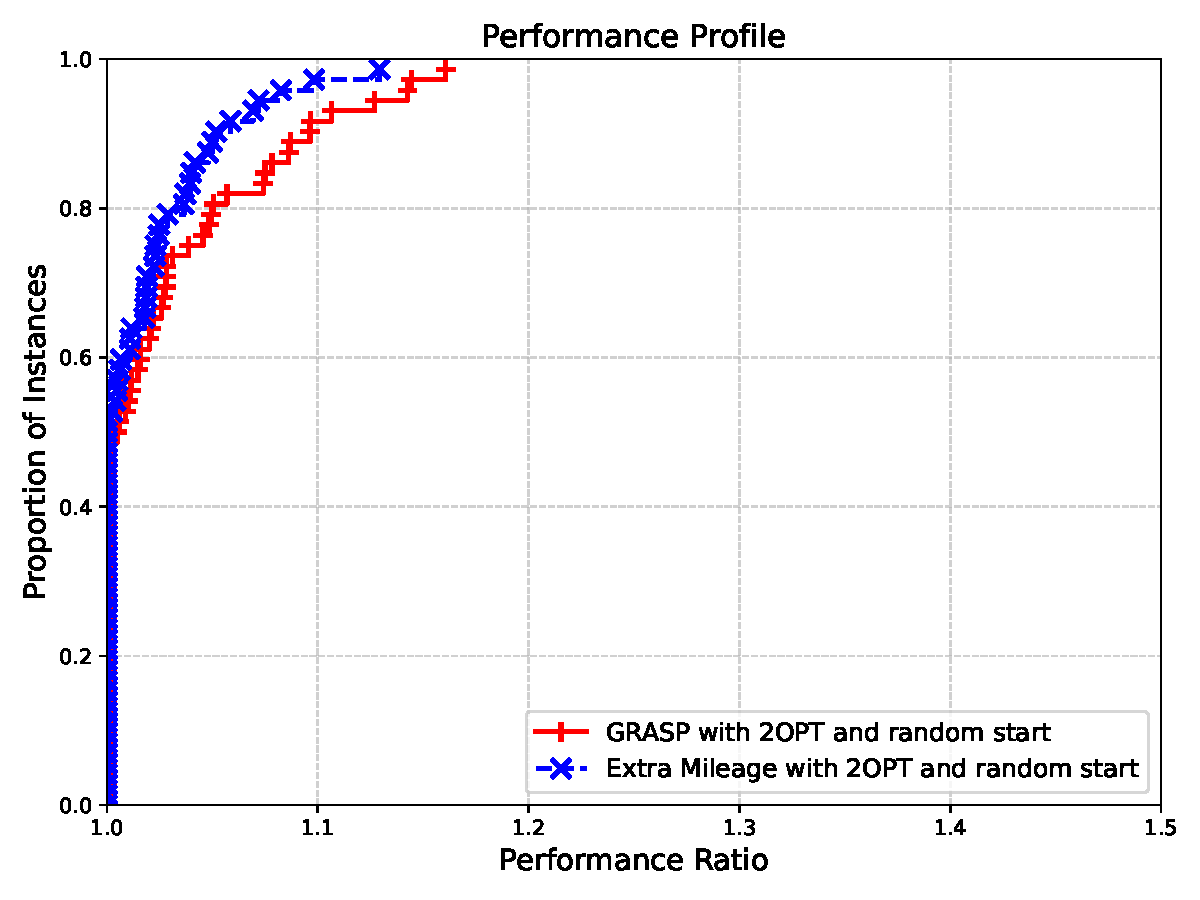
\includegraphics[width=0.8\textwidth]{plots/grasp_vs_extra.pdf}
	\caption{Performance comparison between GRASP and Extra Mileage heuristics on various TSP instances. The graph shows solution quality (as percentage deviation from optimal) for different problem sizes.}
	\label{fig:grasp_vs_extra_mileage}
\end{figure}

The graph in \ref{fig:grasp_vs_extra_mileage} shows the performance of the two heuristics on various randommly generate TSP instances,. 
The results indicate that both heuristics perform similarly, with the Extra Mileage heuristic showing slightly better performance on most instances.


\subsection{Heuristic Algorithms with Different Starting Points}
In this section we will compare the performance of the GRASP and Extra Mileage heuristics with different starting points,
both fixed and random. The starting point in some heuristic may be an influental factor on the quality of the final solution computed by the algorithm, 
it is then interesting to see how the two different approaches differ in terms of performance.

\begin{figure}[!ht]
	\centering
	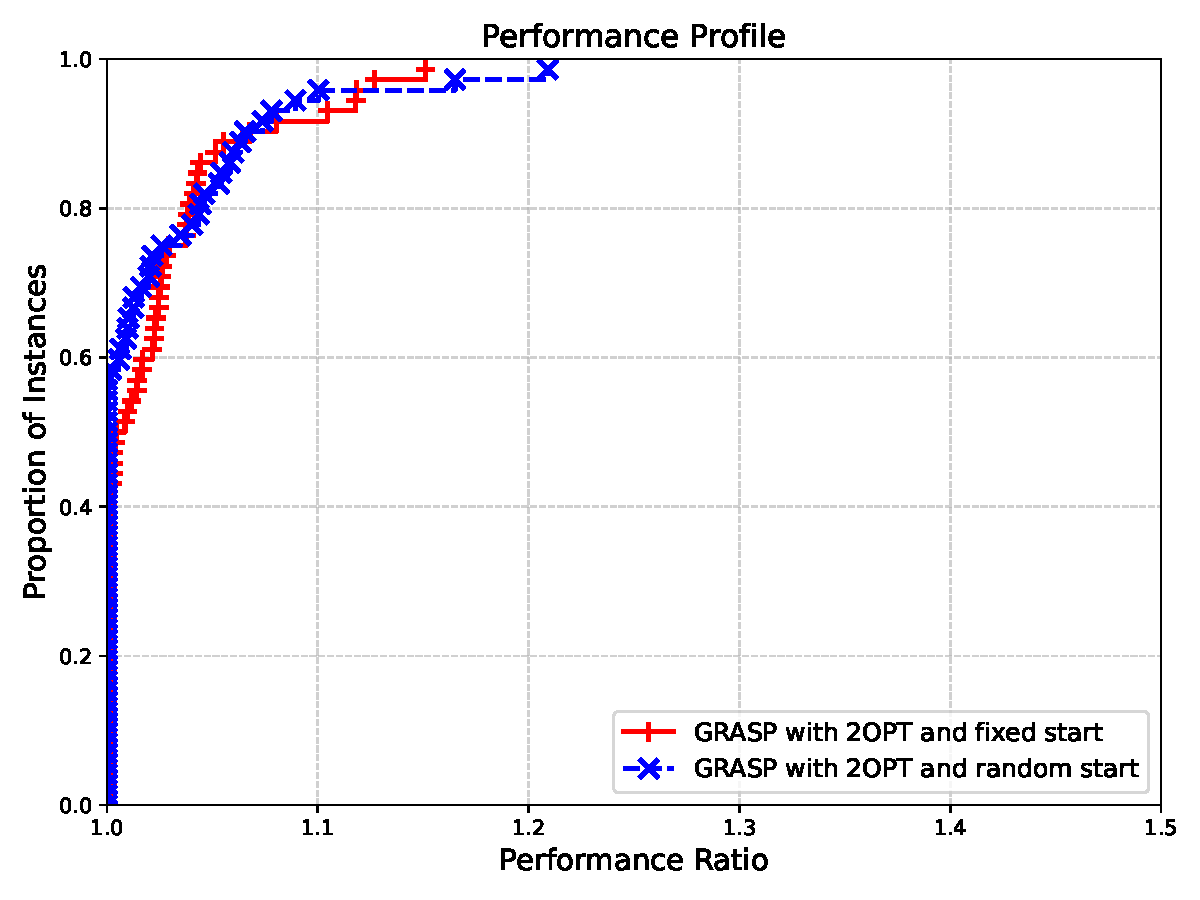
\includegraphics[width=0.8\textwidth]{plots/fixed_vs_random_start.pdf}
	\caption{Performance profiler for GRASP and Extra Mileage heuristics with different starting points (fixed vs random) on a set of random TSP instances.}
	\label{fig:grasp_vs_extra_mileage_starting_points}
\end{figure}
The results indicate that both heuristics perform similarly with fixed and random starting points, 
with the Extra Mileage heuristic showing slightly better performance on larger instances.

\subsection{Tabu Search with Different Tabu List Sizes}
Another interesting aspect of the Tabu Search metaheuristic is the size of the tabu list, which can have a significant impact on the performance of the algorithm.
In this section we will compare the performance of the Tabu Search metaheuristic with different tabu list sizes (10, 20 and 30).

\begin{figure}[!ht]
	\centering
	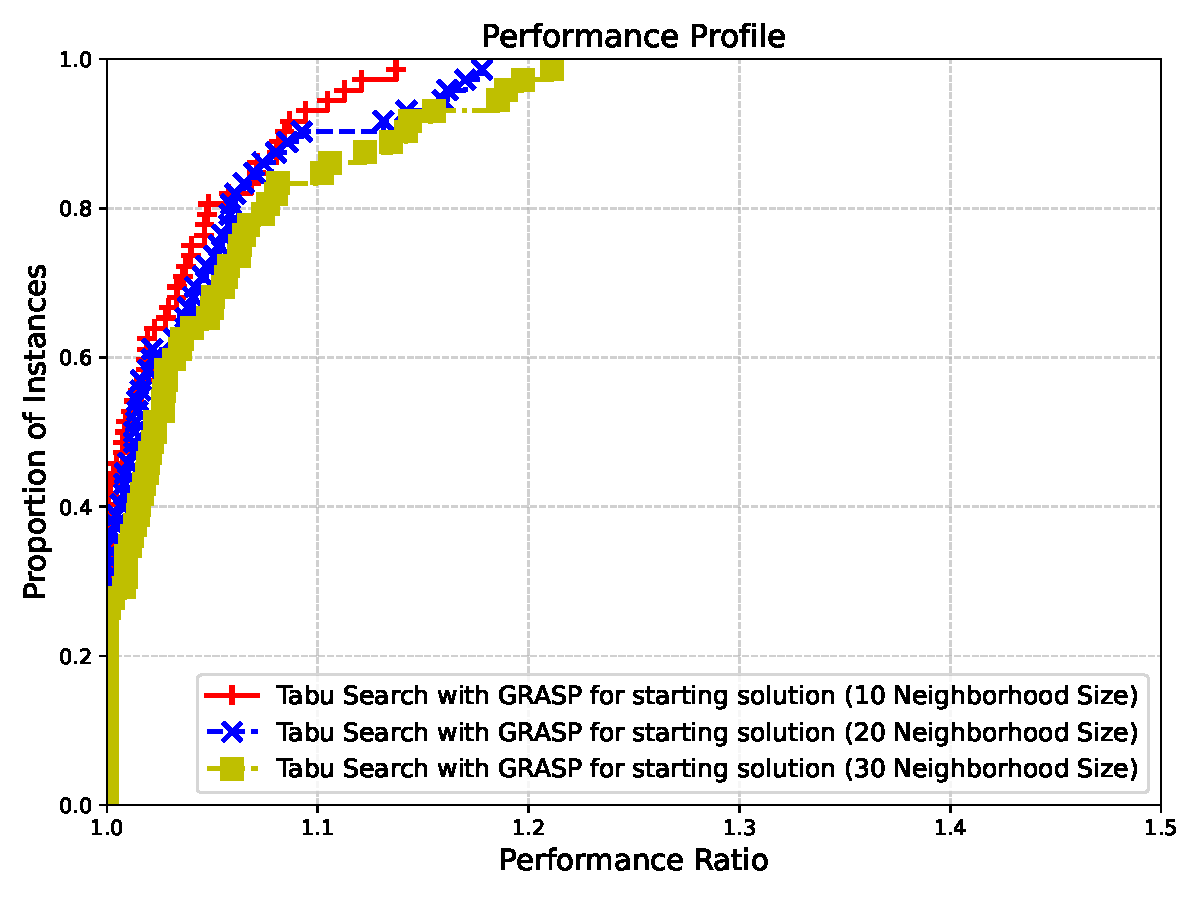
\includegraphics[width=0.8\textwidth]{plots/tabu_variable_neighbourhhod.pdf}
	\caption{Performance profiler for Tabu Search metaheuristic with different tabu list sizes over a set of random TSP instances.}
	\label{fig:tabu_search_tabu_list_sizes}
\end{figure}

The results indicate that the tabu search performs better with larger tabu list sizes, 
with a lower percentage deviation from the optimal solution on larger instances.

\subsection{Heuristic Algorithms vs Metaheuristic}
Now we will take a look at a straight up comparison between the GRASP, Extra Mileage heuristics, and the Tabu Search metaheuristic: 

\begin{figure}[!ht]
	\centering
	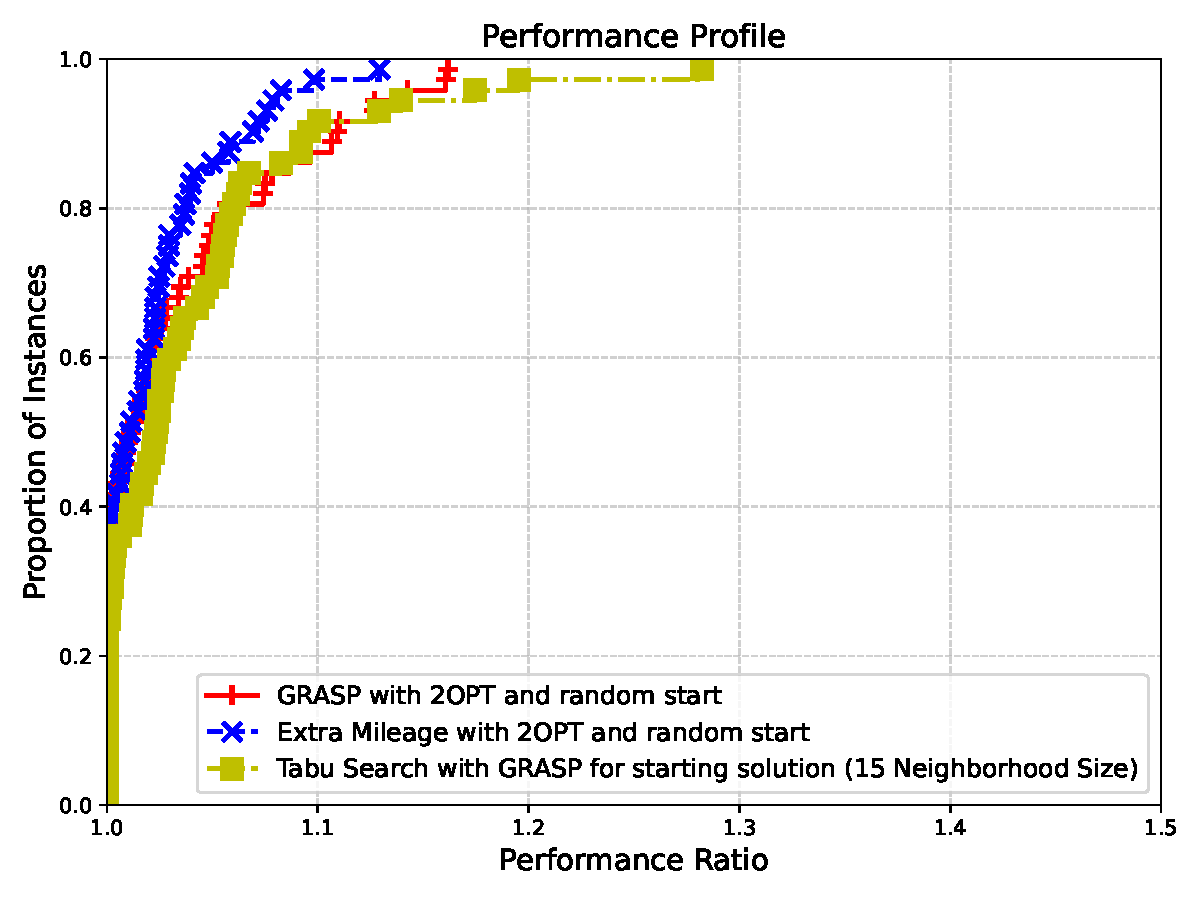
\includegraphics[width=0.8\textwidth]{plots/grasp_extra_tabu_2.pdf}
	\caption{Performance profile comparing GRASP, Extra Mileage heuristics, and Tabu Search metaheuristic on random TSP instances.}
	\label{fig:grasp_vs_extra_mileage_vs_tabu}
\end{figure}

The results indicate that the Tabu Search metaheuristic outperforms both heuristics on larger instances, with a lower percentage deviation from the optimal solution.
\subsection{CPLEX Solver Performance Benchmark}
Finally, we will take a look at the performance of the CPLEX solver on the same set of well known TSP instances. Here we list the results of the implementation of the branch and cut method using 
the CPLEX solver, listing the final cost of the solution, the time taken to solve the problem, and the number of nodes explored by the solver.
\begin{table}[!ht]
	\centering
	\begin{tabular}{|l|l|r|r|}
	\hline
	\textbf{Instance} & \textbf{Method} & \textbf{Cost} & \textbf{Time (s)} \\
	\hline
	a280\_1.tsp & CPLEX Branch and cut & 2586.770 & 20.564 \\
	ali535\_1.tsp & CPLEX Branch and cut & 2009.447 & 313.754 \\
	att48\_1.tsp & CPLEX Branch and cut & 33523.709 & 1.574 \\
	att532\_1.tsp & CPLEX Branch and cut & 86742.422 & 559.105 \\
	a280\_1.tsp & CPLEX Calback approach & 2586.770 & 17.049 \\
	ali535\_1.tsp & CPLEX Calback approach & 2009.447 & 340.157 \\
	att48\_1.tsp & CPLEX Calback approach & 33523.709 & 0.269 \\
	att532\_1.tsp & CPLEX Calback approach & 86742.422 & 829.870 \\
	a280\_1.tsp & CPLEX Branch and cut with Local Branching & 2586.770 & 15.555 \\
	ali535\_1.tsp & CPLEX Branch and cut with Local Branching & 2009.447 & 528.347 \\
	att48\_1.tsp & CPLEX Branch and cut with Local Branching & 33523.709 & 1.039 \\
	att532\_1.tsp & CPLEX Branch and cut with Local Branching & 86742.422 & 1039.645 \\
	a280\_1.tsp & CPLEX Callback approach with Hard fixing  & 2586.770 & 15.012 \\
	ali535\_1.tsp & CPLEX Callback approach with Hard fixing  & 2009.447 & 418.219 \\
	att48\_1.tsp & CPLEX Callback approach with Hard fixing  & 33523.709 & 0.337 \\
	att532\_1.tsp & CPLEX Callback approach with Hard fixing  & 86742.422 & 1342.287 \\
	\hline
	\end{tabular}
	\caption{CPLEX solver performance on well known TSP instances, showing the final cost of the solution, time taken to solve the problem, and number of nodes explored by the solver.}
	\label{tab:cplex_performance}
\end{table}

The results indicate that the CPLEX solver is able to solve the TSP instances in a reasonable amount of time, with the callback approach and the branch and cut method with local branching
showing the best performance on larger instances. The hard fixing approach also shows good performance,
but it is slightly slower than the other two approaches. 
\newpage


\section{Conclusion}
This thesis has explored and implemented a variety of approaches for solving the Traveling Salesman Problem, ranging from classical heuristics to sophisticated metaheuristics and modern mathheuristics. Through our extensive computational experiments and analysis, several key insights emerge:

\subparagraph{Key Findings}
Heuristic Performance: Our implementation and benchmarking of GRASP and Extra Mileage heuristics demonstrated that both approaches provide good-quality solutions, with Extra Mileage showing slightly better performance on larger instances. The 2-opt refinement procedure proved to be an essential component for improving solution quality across all methods.

Metaheuristic Superiority: The Variable Neighborhood Search consistently outperformed other approaches, particularly on larger problem instances. This confirms the value of systematically exploring multiple neighborhood structures to escape local optima.

Parameter Sensitivity: The tabu search algorithm showed significant sensitivity to its tabu list size parameter, with larger list sizes generally yielding better results on complex instances. This highlights the importance of proper parameter tuning in metaheuristic implementation.

Mathheuristic Efficiency: The integration of mathematical programming with heuristic approaches through hard fixing and local branching demonstrated how we can effectively balance exploration and exploitation in the solution space. These approaches provided an efficient way to tackle larger instances that would be intractable for pure exact methods.

Starting Solution Impact: Our experiments with different starting points revealed that while initialization can affect performance, robust metaheuristics can largely overcome poor starting solutions through their search mechanisms.

\subparagraph{Final Remarks}
The TSP remains a fundamental problem in combinatorial optimization with wide-ranging applications. This work has demonstrated the practical effectiveness of 
implementing various solution approaches in the C programming language with CPLEX integration. Our implementations show that while exact methods struggle with large instances, 
well-designed heuristics, metaheuristics, and mathheuristics can provide high-quality solutions in reasonable computational time.

The complementary nature of the different approaches highlights the value of having a diverse algorithmic toolkit when tackling complex optimization problems. 
By understanding the strengths and limitations of each method, practitioners can select the most appropriate approach based on their specific problem characteristics and computational resources.

\newpage

\section{Appendix}
\subsection{Implementation Details}
The implementation of the algorithms described in this thesis is available on GitHub at the following link: \url{https://github.com/yfbenkhalifa/TSP-Optimization-solvers}.

\newpage

\bibliographystyle{alpha}
\bibliography{sample}

\end{document}